\section{Empirical Results and Engineering}
\subsection{Development controls and numerical replay}
The historical smoke scored 9/16; the separate original development baseline scored 11/32. Runtime gripper thresholds 0.4/0.6 scored 18/32 and 15/32, with nominal fix/break counts 14/7 and 9/5; selection chose 0.4. These controls establish neither WSP gains nor a motor-versus-perception advantage.

\begin{figure}[t]
\centering
\begin{minipage}[t]{0.48\linewidth}
\vspace{0pt}\small\captionsetup{type=table}
\caption{Measured unedited-policy evidence. Development calibration is a runtime control, not WSP.}
\label{tab:results}
\begin{tabularx}{\linewidth}{@{}Xr@{}}
\toprule
Quantity & Observation \\
\midrule
Historical smoke: successes / episodes & 9 / 16 \\
Fresh development base ($\tau=0.5$) & 11 / 32 \\
Runtime control ($\tau=0.4$) & 18 / 32 \\
Runtime control ($\tau=0.6$) & 15 / 32 \\
Identity replay: exact / checked & 3 / 3 \\
Historical-action replay: max. error & 0.00683 \\
\bottomrule
\end{tabularx}

\medskip
\caption{Final controls: 64 paired slots each. F/B: nominal fixes/breakages. *Reuses the original identity reference.}
\label{tab:final}
\begin{tabularx}{\linewidth}{@{}Xrr@{}}
\toprule
Control & Base / candidate & F / B \\
\midrule
Fixed16 identity & 24 / 27 & 16 / 13 \\
Original identity & 26 / 23 & 17 / 20 \\
Original gripper 0.4 & 23 / 36 & 21 / 8 \\
Original repeat* & 26 / 35 & 21 / 12 \\
\bottomrule
\end{tabularx}

\end{minipage}\hfill
\begin{minipage}[t]{0.49\linewidth}
\vspace{0pt}\centering
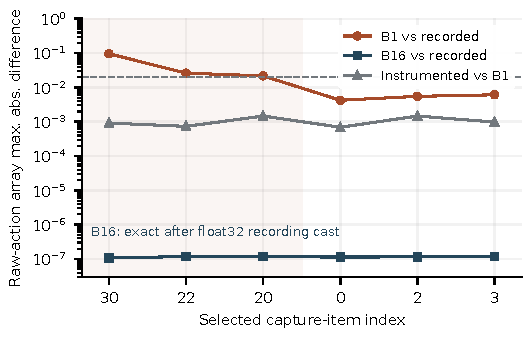
\includegraphics[width=\linewidth]{figures/batch_shape_replay.pdf}
\caption{Six requests from five episodes: three largest failed-capture errors (shaded) and first three passing items. Raw-array errors precede the recording cast; B16 is exact at float32 precision. Dashed line: fixed 0.02 gate. This selected sample does not estimate error frequency.}
\label{fig:smoke}
\end{minipage}
\end{figure}

Identity loading verified all 18 slices and reproduced three actions exactly; historical error was at most 0.006835. A later 32-item single-request capture failed parity (0.09474); four- and 16-item captures passed. Failed arrays remained archived and accessible, but an external audit excluded their use in the reported edit.

On six selected requests (Figure~\ref{fig:smoke}), native B16 reproduced historical chunks after the recording cast; B1 differed by up to 0.09566, with instrumentation adding at most 0.001465. Repeat/identity controls were exact. B16 duplicated one input, not the original mixed packet. No threshold-0.5 gripper flips occurred in 90 action rows. Batch sensitivity here establishes neither its frequency nor closed-loop effects; mixed joint/gripper errors have no single physical unit.

\subsection{Four original discovery runs}
All four runs retained the base policy (Table~\ref{tab:discovery}; Figure~\ref{fig:discovery}). Each run evaluated three proposals; only three of these twelve proposals changed weights. Three nonzero proposals changed 7/2/1 layer-17 rows and 4,412/1,543/791 deployed values, with $\ell_2$ norms 0.02229/0.007959/0.006117. They scored 12/32, 13/32, 13/32, with nominal fixes/breakages 7/6, 9/7, 7/5; each failed preservation. The first projected selected rows away from a passing success-minus-failure activation contrast. A plausible contrast did not establish selective repair.

Nine identity proposals scored 8--20/32. The 20/32 identity cohort had a nominal paired difference 0.2813, with bootstrap interval $[0.0625,0.5000]$, despite zero changes: this is a cohort difference, not an edit effect. Both non-adaptive runs exhausted their activation budgets on failed captures and submitted identities. Their abstention prevents isolating adaptive reasoning under equally usable evidence. Only 24 of 368 charged logical items belonged to fully validated captures; 316 belonged to failed calls and 28 to an unchecked diagnostic. All 384 reserved candidate episodes completed.

\begin{table}[t]
\centering\small
\caption{Original discovery, each against the 11/32 baseline. A/N: adaptive/non-adaptive; 32 episodes per proposal. Nonzero counts proposals that changed deployed weights, not iterations or individual parameters. All runs have three evaluations; other proposals are identities. Capture items belong to validated (V), failed (F), or unchecked (U) whole calls. Min.: driver wall minutes, including reasoning, tools, simulation and waiting.}
\label{tab:discovery}
\begin{tabularx}{\linewidth}{@{}lcrrrX@{}}
\toprule
Run & Successes: p1 / p2 / p3 & Nonzero & Capture items: V / F / U & Min. & Finalist \\
\midrule
A1 & 12 / 14 / 20 & 1 & 20 / 32 / 28 & 61.6 & base \\
N1 & 13 / 17 / 10 & 0 & 0 / 96 / 0 & 50.9 & base \\
A2 & 13 / 14 / 13 & 2 & 4 / 92 / 0 & 67.3 & base \\
N2 & 12 / 8 / 12 & 0 & 0 / 96 / 0 & 47.6 & base \\
\bottomrule
\end{tabularx}

\end{table}

\begin{figure}[t]
\centering
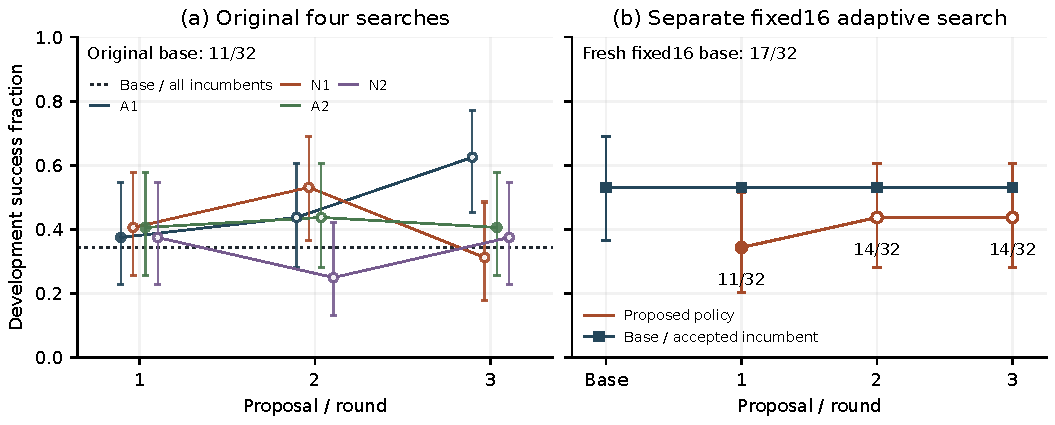
\includegraphics[width=\linewidth]{figures/discovery_summary.pdf}
\caption{Development proposals (open: identity; filled: nonzero edit) and accepted incumbents, with separate baselines and nominal 95\% Wilson intervals. Retained incumbents reuse their score; accepted development scores are nondecreasing by construction. Full restart panels and paired intervals accompany the blog.}
\label{fig:discovery}
\end{figure}

\subsection{Separate fixed16 follow-up}
Offline validation passed on 31 positions from 16 legacy inputs: native repeat, identity, and packet replay were exact; instrumentation error peaked at 0.002464, with zero skips. The fresh 17/32 baseline is not an intervention estimate relative to v1.

The adaptive editor completed three evaluations in 63.43 minutes. All 80 requested activation items passed full-packet parity. It halved the projection of eight layer-17 rows onto a pregrasp success-minus-failure contrast, changing 6,225 bfloat16 values ($\|\Delta\|_2=0.02643$). The candidate scored 11/32 versus 17/32 base, with 5 nominal fixes and 11 breakages, and was rejected. Two identity controls each scored 14/32, with 5/8 and 4/7 fixes/breakages; they disagreed on 10/32 outcomes. The base remained incumbent. Valid capture did not yield an accepted edit or eliminate rollout variability; one run cannot establish a causal comparison with v1.

Held-out identities disagreed on 29/64 fixed16 and 37/64 original-runtime outcomes despite unchanged weights (Table~\ref{tab:final}). Differences were $+0.0469$ and $-0.0469$, with nominal intervals $[-0.1250,0.2031]$ and $[-0.2344,0.1406]$. Round labels share estimates; rejected edits were not substituted. The gripper control scored 36/64 versus 23/64: difference $+0.2031$, interval $[0.0469,0.3594]$. Yet the extra unchanged repeat scored 35/64 versus its reused 26/64 reference: $+0.1406$, interval $[-0.0313,0.3125]$. It had 21/12 nominal fixes/breakages. These correlated repeats and nominal pairing qualify the gripper contrast; its runtime adjustment is not WSP.


\subsection{Repeatability and implementation limits}
A post-hoc first-request audit of all 64 fixed16 identity pairs found identical joint/gripper state and seeds, but different images and actions. Median per-image mean absolute differences were 0.949/2.546 external/wrist intensity units (0--255). Of 960 planned gripper commands, 31 differed across threshold 0.5, spanning seven pairs. This audit isolates neither the source of variability nor perceptual versus motor failures.

An isolated Isaac Sim 6.0.1.0 / Isaac Lab 3.0.0b2.post1 setup used two RTX 4090s, post-bfloat16 support checks, and private RAM checkpoint staging for disk pressure. Simulator-version equivalence remains untested; reproducible setup, validation, and costs accompany the blog.

Post-freeze diagnostics completed 24/16 native forwards for v1/v2 after a separate preallocation-only correction; initial attempts failed allocation. Repeat, identity, and restoration controls were exact. All four edits changed actions on 32 first requests per runtime, each with zero binary gripper flips among 480 planned actions. V1 used new batches; v2 preserved recorded packets. These fixed-input effects do not establish closed-loop gains.

Misused condition-group names caused 62 false yellow-block wrong-object annotations across 28 original baseline episodes, including all 11 successes. Terminal success uses a separate predicate. Editors saw unvalidated logs; their influence is unknown. Both frozen runtimes retain the bug.
